\documentclass[12pt]{report} % A betűméret 12-re és a dokumentum típus jelentés-re állítása.

\def\magyarOptions{defaults=hu-min} % Konfigurálja a magyar nyelvi beállításokat minimális szabályokkal.

\usepackage[magyar]{babel} % A magyar nyelvi csomag betöltése.
\usepackage[T1]{fontenc} % A kimeneti karakterkódolás T1-re állítása.
\usepackage{times} % A Times New Roman betűtípus beállítása.
\usepackage[utf8]{inputenc} % A karakterkódolás UTF8-ra állítása.
\usepackage{fancyhdr} % A fejlécekhez és a láblécekhez használt csomag.
\usepackage{graphicx} % A képek beillesztéséhez szükséges csomag.
\usepackage{titlesec} % A címformázáshoz szükséges csomag.
\usepackage{parskip} % Kikapcsolja az automatikus paragrafus bekezdéseket.
\usepackage{setspace} % A sortávolság beállításához szükséges csomag.
\usepackage{amsmath} % A matematikai képletekhez szükséges csomag.
\usepackage{xcolor} % A színezéshez szükséges csomag.
\usepackage{float} % Az ábrák pontos elhelyezéséhez szükséges csomag.
\usepackage{csquotes} % A nyelvfüggő szövegekhez szükséges csomag.
\usepackage[hidelinks]{hyperref} % A linkekhez szükséges csomag.
\usepackage[backend=biber, style=numeric, sorting=none]{biblatex} % Az irodalmak számozott hivatkozásához szükséges csomag.
\usepackage[a4paper, left=25mm, top=25mm, right=25mm, bottom=25mm]{geometry} % PDF-hez igazított, szimmetrikus 2,5 cm margók minden oldalon.

\addbibresource{references.bib} % Az irodalomjegyzék forrásainak megadása.

\renewcommand*{\bibfont}{\normalfont\fontsize{10}{12}\selectfont} % A betűméret 10-re, a sormagasságot pedig 12-re állítja az irodalomjegyzékben.

\setlength\bibitemsep{\baselineskip} % Az irodalomjegyzék sortávolságának beállítása.

% A magyar irodalomjegyzék beállítása.
\DefineBibliographyStrings{magyar}{
  url = {Elérhetőség:},
  urlseen = {Utolsó megtekintés dátuma:}
}

\DeclareFieldFormat{url}{\\\bibstring{url}\addcolon\space\href{#1}{\textcolor{blue}{\underline{#1}}}} % Megformázza az URL-t az irodalomjegyzékben.

\DeclareFieldFormat{urldate}{\\\bibstring{urlseen}\addcolon\space#1} % Megformázza a megtekintés dátumát az irodalomjegyzékben.

\onehalfspacing % A másfeles sortávolság beállítása.

\setlength{\headheight}{14.5pt} % Növeljük a fejléc magasságát.

\begin{document} % A dokumentum kezdete.

% A fejezetek formázásának módosítása.
\titleformat{\chapter}[hang] % Ez biztosítja a hagyományos elrendezést.
  {\normalfont\huge\bfseries} % A fejezet címe nagy méretű, félkövér betűtípussal jelenik meg.
  {\thechapter.}{1em}{} % A fejezet száma ponttal elválasztva jelenik meg, a cím közvetlenül utána következik.

\titlespacing*{\chapter}{0pt}{-20pt}{\baselineskip} % A fejezetek előtti és utáni térközök beállítása.

% A fejezetek első oldalának stílusának testreszabása.
\fancypagestyle{plain}{
    \fancyhf{} % Törli az alapértelmezett fejlécet és láblécet.
    \fancyhead[L]{Titkosítási módszerek a jövő blokkláncai számára} % A fejléc bal oldalára a diplomamunka címének elhelyezése.
    \fancyfoot[R]{\thepage} % A lap számát a lábléc jobb oldalra rakja.
}

\pagestyle{fancy} % A többi oldalnak a stílusának testreszabása.
\fancyhf{} % Törli az alapértelmezett fejlécet és láblécet.
\fancyhead[L]{Titkosítási módszerek a jövő blokkláncai számára} % A fejléc bal oldalára a diplomamunka címének elhelyezése.
\fancyfoot[R]{\thepage} % A lap számát a lábléc jobb oldalra rakja.

\thispagestyle{empty} % Erről az oldalról törli a fejlécet és láblécet.

\begin{center} % Vízszintesen középre igazítja a tartalmat.
    {\Large\bf Szegedi Tudományegyetem}\\ % Nagy és félkövér szöveg.
    \vspace{0.5cm} % Függőleges térköz beszúrása.
    {\Large\bf Informatikai Intézet}\\ % Nagy és félkövér szöveg.
    \vspace*{8.5cm} % Függőleges térköz kötelező beszúrása.
    {\Huge\bf SZAKDOLGOZAT}\\ % Óriási és félkövér szöveg.
    \vspace*{10cm} % Függőleges térköz kötelező beszúrása.
    {\Large\bf Molnár Gábor Ádám}\\ % Nagy és félkövér szöveg.
    \vspace*{0.6cm} % Függőleges térköz kötelező beszúrása.
    {\Large\bf 2025} % Nagy és félkövér szöveg.
\end{center} % A középre igazított blokk vége.

\newpage % Új oldalt kezd.

\thispagestyle{empty} % Erről az oldalról törli a fejlécet és láblécet.

\begin{center} % Vízszintesen középre igazítja a tartalmat.
    \vspace*{1cm} % Függőleges térköz kötelező beszúrása.
    {\Large\bf Szegedi Tudományegyetem}\\ % Nagy és félkövér szöveg.
    \vspace{0.5cm} % Függőleges térköz beszúrása.
    {\Large\bf Informatikai Intézet}\\ % Nagy és félkövér szöveg.
    \vspace*{3.8cm} % Függőleges térköz kötelező beszúrása.
    {\LARGE\bf Titkosítási módszerek a jövő blokkláncai számára}\\ % Nagy és félkövér szöveg.
    \vspace*{3.6cm} % Függőleges térköz kötelező beszúrása.
    {\Large Szakdolgozat}\\ % Nagy szöveg.
    \vspace*{4cm} % Függőleges térköz kötelező beszúrása.
    {\large % Nagy szöveg.
    \begin{tabular}{c@{\hspace{4cm}}c} % Két oszlop 4 cm-es térközzel.
    \emph{Készítette:} &\emph{Témavezető:}\\ % Dőlt címkék.
    \textbf{Molnár Gábor Ádám} &\textbf{Dr. habil. Kertész Attila}\\ % Félkövér nevek.
    informatika szakos &egyetemi docens\\ % Szak és beosztás kiírása.
    hallgató& % Az utolsó sorban nincs második oszlopbeli tartalom.
    \end{tabular}
    }\\
    \vspace*{2.5cm} % Függőleges térköz kötelező beszúrása.
    {\Large % Nagy szöveg.
    Szeged % Szeged kiírása.
    \\ % Új sor
    \vspace{2mm} % Függőleges térköz beszúrása.
    2025 % Az évszám kiírása.
    }
\end{center} % A középre igazított blokk vége.

\tableofcontents % Tartalomjegyzék beszúrása

\chapter*{Feladatkiírás} % Sorszám nélküli fejezet létrehozása.
\addcontentsline{toc}{chapter}{Feladatkiírás} % A fejezet hozzáadása a tartalomjegyzékhez.

A felhő és blokklánc-alapú platformok iránti érdeklődés jelentősen megnőtt, ami az ellátási láncok racionalizálásában, a nyomon követhetőség javításában, a kereskedelem egyszerűsítésében és a pénzügyi tranzakciók hatékonyabbá tételében rejlő lehetőségüknek köszönhető. Ez a fellendülés a Bitcoin egyre népszerűvé válásával kezdődött, rávilágítva a régebbi blokklánc platformok energiafogyasztással és késleltetéssel kapcsolatos kihívásaira.

A modern blokklánc platformok ezen problémák megoldását célozták meg, és hatékonyabb módszereket nyújtanak a különböző üzleti alkalmazásoknak.

A blokklánc rendszerek egy fontos eleme a titkosítási algoritmusok alkalmazása. Napjainkban az SHA-256 algoritmust használják a tranzakciók és a hálózati kommunikáció biztonságossá tételére, de a szakirodalomban számos egyéb algoritmust is javasoltak bizonyos tulajdonságok javítására (például titkosítás erőssége, gyorsasága).

A szakdolgozó feladata ezen szakirodalmi megoldások áttekintése, tanulmányozása, különös tekintettel a jövő blokklánc rendszerei és poszt-kvantum megoldásai tekintetében. További cél egy saját titkosítási algoritmus kifejlesztése és összehasonlítása teljesítménymérések elvégzésével, a szakirodalomban elérhető közeli megoldásokkal összevetve.

\chapter*{Tartalmi összefoglaló} % Sorszám nélküli fejezet létrehozása.
\addcontentsline{toc}{chapter}{Tartalmi összefoglaló} % A fejezet hozzáadása a tartalomjegyzékhez.

\section*{A téma megnevezése} % Sorszám nélküli alcím létrehozása.

Titkosítási módszerek a jövő blokkláncai számára és ezek összehasonlítása.

\section*{A megadott feladat megfogalmazása} % Sorszám nélküli alcím létrehozása.

A feladat a különböző titkosítási algoritmusok összehasonlítás, különböző szempontok alapján. Továbbá egy saját algoritmus fejlesztése és összehasonlítás a már létező és aktívan használt algoritmusokkal.

\section*{Megoldási mód} % Sorszám nélküli alcím létrehozása.

Egy grafikus felülettel rendelkező alkalmazás elkészítése, amelyen könnyedén lehet futtatni Unit teszteket a különböző algoritmusokra. Valamint alkalmas az eredmények áttekinthető kimutatására.

\section*{Alkalmazott eszközök, módszerek} % Sorszám nélküli alcím létrehozása.

Az alkalmazás egy ASP.NET Core webalkalmazás lett. A tesztek futtatására az NUnit csomagot használja, a megjelenítésre pedig a Chart.js csomagot. Az eredményeket egy SQLite adatbázisban tárolja.

\section*{Elért eredmények} % Sorszám nélküli alcím létrehozása.

Egy teljesen működő és tesztelésre alkalmas webalkalmazás. Továbbá egy saját szimmetrikus titkosító algoritmus C\# megvalósítása.

\section*{Kulcsszavak} % Sorszám nélküli alcím létrehozása.

C\#, ASP.NET Core, NUnit, Chart.js, blokkláncok, kriptográfia

\chapter{Bevezetés} % Sorszámozott fejezet létrehozása.

\section{Motiváció} % Sorszámozott alcím létrehozása.

Mindig is akartam valami maradandót alkotni. Valami olyat, ami nem csak egy kézzel fogható tárgy. Valamit, amire mindig büszkén tudok visszanézi. Még akkor is ha nem a legtökéletesebb munkám lenne. Egy olyan eszmei értéket, amit bárki tud használni kedve szerint. Talán úgy ahogy én elképzeltem. De az is lehet, hogy csak alapul használják és javítanak rajta. Már ez is nagy öröm lenne számomra. Mert látnám, hogy mások szerint is jól sikerült az alkotásom, hiszen mi másért használnak?

Ez volt az hajtóerő, aminek hatására elkezdtem egy saját titkosító algoritmust fejleszteni. Hiszen másoknak is sikerült már előttem. Nem is egy ilyen algoritmus van amit a mindennapi életünkben szinte állandó jelleggel használunk. Mégsem mondjuk soha sem egy algoritmusra, hogy ez a legjobb, vagy éppen az a másik. Ilyen tekintetben szerintem ezek az algoritmusok egy kicsit misztikus dolgok. Mivel nehéz eldönteni, hogy kettő közül melyik a jobb. Mert mindig az a kérdés merül fel, hogy milyen értelemben jobb?

Ebben a szakdolgozatban megpróbálom részletesen összehasonlítani az ismertebb titkosító algoritmusokat különböző szempontok alapján. Lehetőleg ezzel érthetőbbé válik ezen algoritmusok világa egy átlagos ember vagy fejlesztő számára. Továbbá kifejtem a saját algoritmusom fejlesztésének folyamatát. Bele érte minden akadályt és nehézséget is, amibe ennek során beleütköztem.

\section{Kriptográfia} % Sorszámozott alcím létrehozása.

Az emberek szeretik biztonságban tudni a bizalmas dolgaikat. Legyen az egy betöréses támadás vagy egyszerű adatküldés esetén. Ez a probléma ihlette meg a kriptográfiai algoritmusokat. Egy ilyen algoritmus egy nyílt szöveget vár bemenetként, majd egy kulcs segítségével egy titkosított szöveget hozz létre a kapott szövegből. Ez minden kriptográfiai algoritmus alapelve.

Fontos kiemelni, hogy a kriptográfiai algoritmusokat \cite{szteCryptography} több módon tudjuk csoportosítani. Az első lehetőség az, hogy az elvégzett műveletek alapján csoportosítjuk őket. Így megkülönböztetjük a keverő, helyettesítő és produkciós titkosító algoritmusokat.

A keverő algoritmusoknál a titkosított szöveg egyszerűen az eredeti szöveg karaktereinek permutációja. Értelem szerűen ez nem nyújtja a legnagyobb biztonságot. Tekintve, hogy a permutáció lehet akár az eredeti szöveg is. Igaz, ez inkább a rövid szövegek esetén valószínűbb, hogy bekövetkezik.

A helyettesítő algoritmusok a nyílt szöveg karaktereit a titkosított szöveg karaktereivel helyettesítik. Ez történhet egyesével vagy akár blokkokban is. Ezek az algoritmusok már nagyobb biztonságot nyújtanak, mint a keverő algoritmusok. De ez sem egy új keletű dolog, a németek Enigma gépe is ezen az elven alapszik. A ki jártasabb a történelemben az tudja, hogy nagyon sokáig nem tudták feltörni az Enigmával küldött üzeneteket.

A produkciós algoritmusok pedig a kettő elv kombinációján alapszanak. Ezek bizonyultak eddig a leghatékonyabb titkosítási módnak. A napjainkban használt algoritmusok is ide tartoznak. A szakdolgozat keretein belül ilyen algoritmusokról lesz részletesebben szó.

A másik felosztási lehetőség, az algoritmus kulcsa szerint történik. Ebben a felosztásban megkülönböztetjük a szimmetrikus és aszimmetrikus kulcsú algoritmusokat. Vitatható, hogy van egy harmadik csoport is, amiben a hasító algoritmusok vannak.

A szimmetrikus kulcsú algoritmusok onnan kapták a nevüket, hogy ugyan azt a kulcsot használjuk titkosításnál és visszafejtésnél is. Ilyenkor mindkét félnek a birtokában van a kulcs. Ennek az a veszélye, hogy a kulcs kiszivároghat. Ha ez megtörténik, akkor innentől kezdve bári el tudja olvasni a titkosított szövegeket.

Az aszimmetrikus kulcsú algoritmusok ezt úgy próbálták orvosolni, hogy két különböző kulcs van. Az egyiket a szöveg titkosításánál kell használni, a másikat pedig a visszafejtésénél. Így csökken az illetéktelen visszafejtés veszélye, mert az ehhez szükséges kulcsot sosem kell megadni senkinek. Ezeket az algoritmusokat sok helyen használjuk manapság. Például végpontok közötti titkosításos üzenetküldésnél.

Az utolsó csoport a hasító algoritmusok. Ezek oly módon titkosítják a nyílt szöveget, hogy azt nem lehet visszafejteni. Egyértelmű, hogy ezek az algoritmusok nem a legmegfelelőbbek titkosított üzenetek küldésére. Hiszen a fogadó fél nem tudja, hogy mi is volt az üzenet eredeti tartalma. Ezen algoritmusok egyik elterjedt felhasználási módja a digitális aláírás. Melynek segítségével a kapott tartalom eredetiségét lehet ellenőrizni.

A szakdolgozat többi részében konkrét szimmetrikus, aszimmetrikus és hasító algoritmusokról lesz szó. Ezek mind produkciós algoritmusok. A keverő és helyettesítő algoritmusokkal külön nem foglalkozom ezen projekt keretein belül.

\section{Poszt-kvantum kriptográfia} % Sorszámozott alcím létrehozása.

A kvantumfizika és a kvantummechanika egy elég nehezen értelmezhető tananyag. A szakdolgozathoz csak indirekt módon kapcsolódnak. Mivel a kvantumszámítógépek működése ezeken alapszik. Röviden fogalmazva a kvantumszámítógépek nem egyszerű általános felhasználásra készített számítógépek, hanem inkább különlegesebb feladatok megoldására szolgálnak \cite{sslMarketBlogPostQuantum}. Ehhez természetesen szükség van megfelelő algoritmusokra is.

Az információ biztonság tekintetében a problémát az képzi, hogy a legtöbb manapság titkosításra használt algoritmus gyorsabban feltörhető kvantumszámítógéppel. Értelem szerűen ezzel csökken az algoritmusok által nyújtott biztonság. Szerencsére ma még nem teljesen reménytelen a helyzet. Megfelelő kulcshosszúsággal még mindig elég nagy biztonságot nyújtanak a mostani algoritmusok.

Poszt-kvantum algoritmusoknak nevezzük azokat az algoritmusokat, amelyek ellenállók a kvantumszámítógéppel való támadásoknak. Ilyen például a Crystals-Kyber aszimmetrikus kulcsú algoritmus. Digitális aláírásra pedig Crystals-Dilithium algoritmus.

\section{Blokkláncok} % Sorszámozott alcím létrehozása.

A blokkláncok egy nemrégen megjelent új adatbázis fajta. Céljuk az adatok lehető legbiztonságosabb tárolása egy decentralizált módon \cite{daglarCizmeciBlockchain}. Első hallásra ez egy nagyon hasznos előrelépésnek tűnhet, de sajnos amint minden új technológiának, ennek is vannak problémái. Először is, egy blokklánc úgy tárolja az adatokat, hogy úgy nevezett blokkokba rendezi őket. Majd az elkészült blokkokat hozzá rakja, azaz összeláncolja a már meglévő blokkokkal. Innen kapta a névét a technológia, hiszen a tárolt adatok gyakorlatilag blokkok egymásba fűzött lánca.

Talán a legnagyobb erősségük egyben az egyik hátrányuk is. Ez alatt arra gondolok, hogy a már egyszer hozzá adott blokkot soha sem lehet megváltoztatni. Ez ugyan hatalmas biztonságot nyújt, hiszen azonnal észre lehet venni, ha valaki módosította az adatokat. Ám sajnos ennek a tulajdonságnak köszönhetően nem fogja tudni kiváltani a manapság szinte mindenhol használt relációs adatbázisokat. Tekintve, hogy egy egyszerű jelszó módosítás nem lenne lehetséges, ha a felhasználói fiók egy blokkban lenne tárolva.

A másik nagy előnyük az, hogy decentralizált módon lehet őket tárolni. Ez egy jelentős előrelépés a relációs adatbázisokkal szemben, amiket általában centralizált módon használunk. A decentralizált tárolási mód nagyobb biztonságot add támadásokkal szemben, hiszen az adatok nem egyetlen központosított helyen vannak tárolva. A biztonság további növelése érdekében a blokkokban lévő adatokat még általában titkosítják is. Ez szimmetrikus vagy aszimmetrikus algoritmusokkal is történhet. A láncolásnál pedig hasító algoritmustokat használnak az egyedi azonosítók létrehozásához. A szakdolgozatat szempontjából ezért fontos mind a három fajta titkosító algoritmus.

Végezetül a blokkláncoknak van egy nehézségük, a skálázódás. Ez egy általános probléma a blokkláncokban, bár az oka nem mindig ugyanaz. A Bitcoin-nál például a blokkok méretének korláta okozza. De okozhassa akár a hastó függvény futásához szükséges idő is. Ezért is fontos a blokkláncok számára, hogy a lehető leghatékonyabb algoritmusokat használják. A szakdolgozatnak részben ezek megtalálása a célja. Természetesen nem csak a legmegfelelőbb hasító algoritmust, hanem mind a három fajtából a lehető legjobbat.

\chapter{Felhasznált technológiák} % Sorszámozott fejezet létrehozása.

\section{C\#} % Sorszámozott alcím létrehozása.

Azért választottam a C\# \cite{cSharp} nyelvet, mivel jelenleg is ebben dolgozom a BerényiSoftware Tanácsadó és Szolgáltató Kft. cégnél. Úgy gondolom ebben a nyelvben vagyok a legjártasabb. Már volt szerencsém egy pár alkalmazást elkészíteni benne a cég megbízásából. Ezeknek a pontos részleteibe nem megyek bele, mivel köt a céges titoktartás. A lényeg az, hogy már fejlesztettem benne webalkalmazást, mobilalkalmazást valamint háttér szolgáltatást is. Továbbá ez egyik egyetemi kurzus keretein belül már egy egyszerű játékot is készítettem. Ezért tartom számomra a legalkalmasabb nyelvnek bármilyen jellegű alkalmazás fejlesztésére.

A szakdolgozatot a .NET 8-as verziójában írtam. Amikor elkezdtem a fejlesztést, akkor még ez volt a legfrissebb verzió. Azóta már megjelent a 9-es verzió is. Viszont nem láttam különösebb indokot, hogy átvigyem a projektet az új verzióra. Ezért maradt a 8-as verzión.

\section{ASP.NET Core} % Sorszámozott alcím létrehozása.

Tapasztalataim alapján a manapság leginkább használt C\# alapú webalkalmazás típus egyike az ASP.NET Core \cite{aspNetCore}. Ezen belül megkülönböztetjük a Razor és az MVC fajtát, én inkább az MVC-t szertem használni. Nekem ez a tervezi minta jobban átlátható. Mivel a nyelvet már eldöntöttem, ezért itt már nem volt olyan sok választási lehetőségem. De ez egy cseppet sem zavart. Nincs semmi bajom az ASP.NET Core alkalmazásokkal. Szerintem kifejezetten egyszerűen és gyorsan felépíthetőek. Részben ezért is esett a választásom a webalkalmazásra. Úgy gondolom, hogy ha szükség van egy grafikus felhasználói felületre, akkor fejlesztési sebesség szerint a webalkalmazások a leggyorsabban elkészíthetőek.

\section{NUnit} % Sorszámozott alcím létrehozása.

Tapasztalataim szerint a három leggyakrabban használt Unit teszt csomag C\#-ban az NUnit, xUnit.net és az MSTest. A cég ahol dolgozom, az NUnit-ot \cite{nUnit} használja. Ez nagyban befolyásolta a döntésemet ennél a választásnál. Ugyan még nem kellet különösen foglalkoznom vele a céges munkáim során. Akkor is ezt tartottam a legmegfelelőbbnek. Tekintve, hogy bármikor segítséget tudok kérni a cégnél dolgozó tesztelőktől. Valamint nem gondolom, hogy a cég véletlenül használja pont az NUnit-ot. Hiszen létezik más Unit tesztelésre alkalmas csomag is. Visszatekintve nem bántam meg a választásomat. A használata során semmiféle technikai vagy funkcionalitásbeli problémát nem tapasztaltam.

\section{Chart.js} % Sorszámozott alcím létrehozása.

A Chart.js \cite{chartJs} egy nagyon népszerű JavaScript csomag. Kiválóan alkalmas rengeteg különféle diagram kirajzolására. Legyen az statikus vagy interaktív, támogatja minden a kétféle grafikonfajtát. Ami még nagyon hasznos tud lenni benne, az a lehetőség, hogy akár több különböző grafikonfajtát is megjelenítsen egyetlen diagramon. Ennek a funkciónak én is nagy hasznát vettem. Szerintem egy kiváló választás bármilyen jellegű webalkalmazásban, ahol diagramok megjelenítése szükséges. A használata is egyszerű, egy kezdő programozó is könnyedén tudja integrálni az alkalmazásába. Esetleges elakadás esetén a hivatalos oldalukon elérhető dokumentáció kiváló támpontot nyújthat. A fogalmazásmódja érthető, nem túl bonyolított. Példa kódokat is tartalmaz. Nekem nem sikerült semmilyen megoldhatatlan problémába ütköznöm a csomag használata során. Ezért mindenkinek csak ajánlani tudom.

\section{BouncyCastle.Cryptography} % Sorszámozott alcím létrehozása.

Erre a csomagra azért volt szükség, mert az alap .NET környezetben elég kevés titkosító algoritmus van megvalósítva. Ez volt az első alkalom, hogy BouncyCastle-tól \cite{bouncyCastle} használtam egy csomagot. Egy rövid fórum olvasás után kiderítettem, hogy egy elég jól elfogadott csapatról van szó. Valamint nem is csak C\# nyelvre, hanem Java-ra is fejlesztenek csomagokat. A C\# megvalósításuk teljesen jól működik, nem volt vele semmi probléma. A dokumentációjuk viszont lehetne egy kicsit felhasználó barátabb. Nem mindig találtam meg benne amit kerestem. Én azzal a véleménnyel vagyok, hogy ha egy fórumról gyorsabban megtalálom a nekem szükséges információt, akkor a hivatalos dokumentációnak van még hova fejlődnie. Szerencsére csak egy-két dolog volt, amit meg kellet keresnem a dokumentációban. Mindent összegezve, nem egy rossz csomag. Nem bántam meg, hogy ezt választottam.

\section{Git, GitHub, GitLab} % Sorszámozott alcím létrehozása.

Verziókövetésre Git-et \cite{git} használtam. Leginkább azért, mert ez az egyetlen verziókövető amit ismerek és aktívan használok. Az egyetemen is csak ezt kérték mindig tőlünk. Valamint a cégben is csak ezt használjuk. Nem akartam most egy teljesen új verziókövetőt kipróbálni. Ezért maradtam a már jól bevált Git-nél. A projektet feltöltöttem az egyetemi GitLab-ra \cite{gitLab}, hogy a témavezetőm könnyedén hozzáférhessen. A GitLab hibajegy kezelő részét ebben a projektben nem vettem igénybe, mivel egyedül én dolgoztam rajta. A GitFlow-t is feleslegesnek éreztem. A biztonság kedvért a saját GitHub \cite{gitHub} fiókomra is feltöltöttem. Semmi esetre sem szerettem volna elveszíteni az eddigi munkámat. Ezért láttam észerűnek három helyen tartani az egész projekt kódját. Szerencsére nem tapasztaltam hardver problémát a fejlesztés alatt. Egyszer sem kellet a szerveren lévő másolatról újra építeni a projektet. A verziókövetési folyamat zavartalanul és problémamentesen működött.

\chapter{Architekturális terv} % Sorszámozott fejezet létrehozása.

\section{Webalkalmazás} % Sorszámozott alcím létrehozása.

Az elképzelésem az volt, hogy egy webalkalmazásban előre definiált Unit teszteket lehet futtatni a megvalósított algoritmusokra. Sajnos nem láttam egyszerű megoldás arra, hogy a felhasználó futási időben adhasson meg új tesztelési szempontot, azaz egy teljesen új Unit tesztet. Ezért mentem inkább abba az irányba, hogy előre megírt tesztek közül lehet választani a grafikus felületen. Ugyan ez a probléma fennállt az algoritmusoknál is. Itt szintén arra a következtetésere jutottam, hogy muszáj lesz őket előre megvalósítani. A teszteseteknél viszont nem láttam akadályát, hogy a felhasználó a felületen keresztül adjon meg új teszteseteket, vagy kiválasztja a neki éppen szükséges eseteket a már létezők közül. Tehát összegezve, egy olyan webes felültetet akarok készíteni, ahol a felhasználó könnyedén kijelölheti a tesztelési szempontot a neki tesztő tesztesetekre. Majd ezeket a teszteket a szerver lefuttatja, ezzel nem terhelve a felhasználó gépét. Tekintve, hogy itt könnyedén szükség lehet elég jelentő mennyiségű számítási kapacitásra. A kész tesztek eredményeit a szerver eltárolja, amit a felhasználó ezután könnyedén letud kérdezni.

\section{Model-View-Controller} % Sorszámozott alcím létrehozása.

Úgy gondolom, hogy ebben a webalkalmazásban is kiválóan alkalmazható az MVC \cite{mozillaMvc} tervezési minta. Egyértelműen szétválasztaná az alkalmazás rétegeit, ezzel megkönnyítve a tesztelést és a hibakeresét is. Bár ez a fajta strukturálás nagyobb csapatban való fejlesztésnél a leghatékonyabb. Tekintve, hogy a konfliktusok elkerülése lényegesen meggyorsítja a fejlesztés folyamatát. Ami jelentősen könnyebb a minta rétegelésnek köszönhetően. Mivel egyedül dolgozom a projekten, itt ez alapból sem volt probléma. Viszont az átláthatóságot akkor is lényegesen javítja. Valamit megadja az a rugalmasságot, hogy a jövőben lehet akkor egy asztali alkalmazás is készíteni belőle. Hiszen csak a vezérlő réteget kell lecserélni, az alkalmazás többi része érintetlen marad.

\section{Szeparáció} % Sorszámozott alcím létrehozása.

Figyelembe véve, a tervezési minta választásomat és az alkalmazás funkcionalitását. Arra a döntésere jutottam, hogy hasznos lenne az alkalmazás részeit teljesen elkülöníteni egymástól. Lenne egy külön rész a közös komponenseknek, a teszteredményeknek, a teszteknek és magának a webalkalmazásnak. Tekinthessük ezeket egymásra épülő alprojekteknek. Ilyen jellegű elkülönítés jelentősen segíti a projekt átláthatóságát. Valamit az objektum orientált alapelvek betartását is. Továbbá könnyebbé teszi a projekt új funkciókkal való bővítését. Még akkor is ha az egy előre be nem tervezett funkció. Ez a csoportosítás az MVC mintával együtt nagy rugalmasságot add az alkalmazásnak.

\section{Algoritmusok egységesítés} % Sorszámozott alcím létrehozása.

Szeretném, hogy bármilyen titkosító algoritmust le lehessen tesztelni az alkalmazással. Még akkor is ha az algoritmus megvalósítása nem a sajátom. Ezért kell egy módszer, hogy egy már létező algoritmus megvalósítását univerzális módon oda tudjam adni a Unit teszteknek. Tekintve, hogy az alkalmazás nyelve C\#, ezt könnyedén meg lehet oldani interfészekkel.

% Kötelező helyű ábra beszúrása.
\begin{figure}[H]
    \centering % Az ábra középre igazítása.
    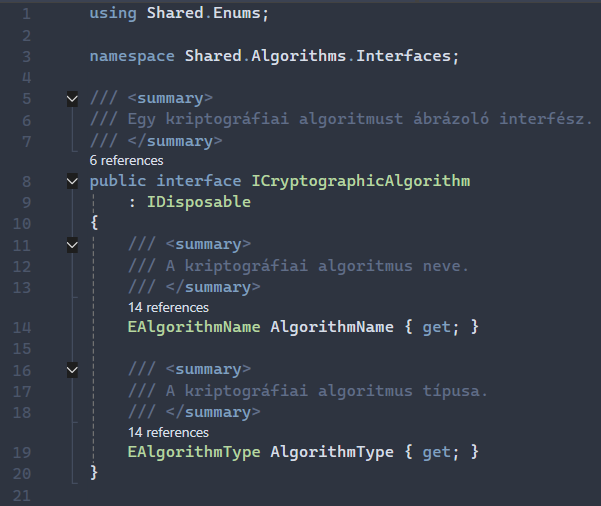
\includegraphics[width=0.8\textwidth]{Figures/ICryptographicAlgorithm.png} % Kép beszúrása.
    \caption{Egy általános algoritmust ábrázoló interfész} % Az ábra neve.
    \label{fig:ICryptographicAlgorithm} % Az ábra referenciája.
\end{figure}

Az én megvalósításom a \ref{fig:ICryptographicAlgorithm} ábrán látható. A kódolási stílusom szerint az interfészek mindig \textit{I} betűvel kezdődőnek, az enumok pedig \textit{E} betűvel. Valamint az XML hozzászólások magyar nyelvűek. Tehát az ábrán látható két tulajdonság egy-egy enum. Az \textit{EAlgorithmName} a projektben definiált algoritmusok neveit tartalmazza. Az \textit{EAlgorithmType} pedig az algoritmusok típusait (szimmetrikus, aszimmetrikus és hasító). Ez az interfész reprezentálja a legmagasabb absztrakciós szint egy algoritmus számára. Ebből származik két már speciálisabb interfész, az \textit{IEncryptionAlgorithm} és az \textit{IHashingAlgorithm}. Értelem szerűen az első ábrázolja a visszafejthető algoritmusokat, a második pedig a visszafejthetetleneket. Az interfészek kódjai a \ref{fig:IEncryptionAlgorithm} és a \ref{fig:IHashingAlgorithm} ábrán láthatóak.

% Kötelező helyű ábra beszúrása.
\begin{figure}[H]
    \centering % Az ábra középre igazítása.
    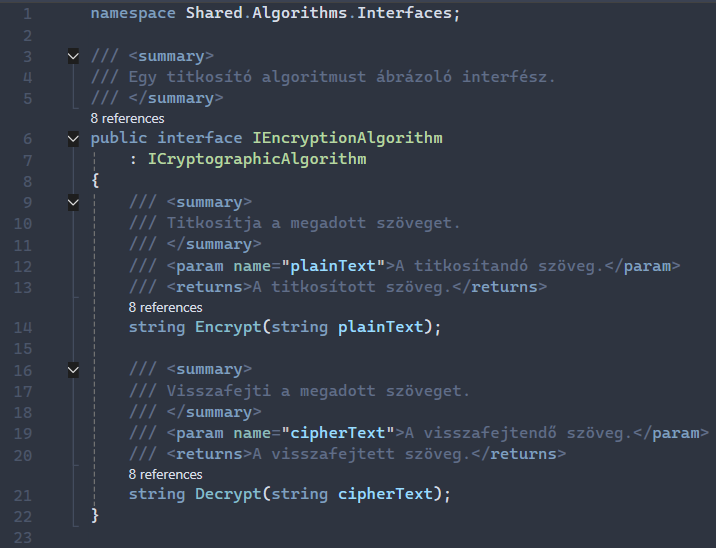
\includegraphics[width=0.8\textwidth]{Figures/IEncryptionAlgorithm.png} % Kép beszúrása.
    \caption{Egy visszafejthető algoritmust ábrázoló interfész} % Az ábra neve.
    \label{fig:IEncryptionAlgorithm} % Az ábra referenciája.
\end{figure}

Az \textit{IEncryptionAlgorithm} felépítésének köszönhetően ábrázolhat egy szimmetrikus vagy aszimmetrikus algoritmust is, szükségtelen két külön interfészt definiálni. Az \textit{IHashingAlgorithm} pedig a hasító algoritmusokat ábrázolja. Ezeknek az interfészeknek köszönhetően bármilyen algoritmust univerzálisan lehet kezelni. Lényegesen könnyebbé téve a Unit tesztek írását.

% Kötelező helyű ábra beszúrása.
\begin{figure}[H]
    \centering % Az ábra középre igazítása.
    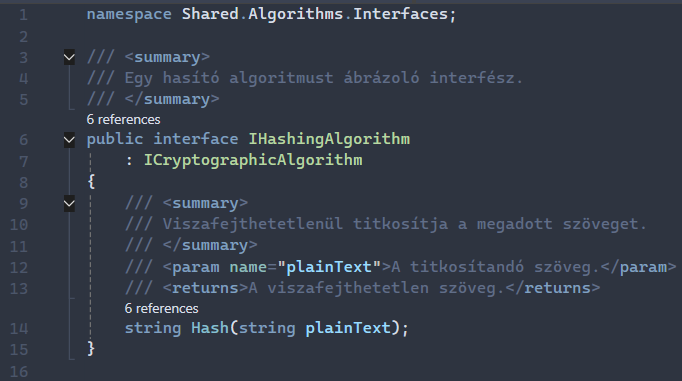
\includegraphics[width=0.8\textwidth]{Figures/IHashingAlgorithm.png} % Kép beszúrása.
    \caption{Egy visszafejthetetlen algoritmust ábrázoló interfész} % Az ábra neve.
    \label{fig:IHashingAlgorithm} % Az ábra referenciája.
\end{figure}

\section{Tesztelt tulajdonságok} % Sorszámozott alcím létrehozása.

Rengetek különböző módon lehetne tesztelni ezeket az algoritmusokat. Viszont a rendelkezésre álló idő korlátozott. Ezért a legjelentősebb tulajdonságok tesztelésére koncentráltam, a memóriahasználat és a futási idő. Ezeket szintén több különböző helyzetben lehet tesztelni. Az eredeti elképzelésben magának az algoritmusnak simán és egy blokkláncba helyezve is mérve lett volna a hatékonysága. Sajnos az utóbbi végül teljesen el lett hagyva, tekintettel a szűkös időkorlátra. Viszont így is egy elég jó képet tudunk kapni az algoritmus hatékonyságáról és a korlátairól. Az interfészeknek köszönhetően pedig ezek teljesen univerzális tesztek minden jelenlegi és jövőbeli algoritmusra.

\section{Adatbázis} % Sorszámozott alcím létrehozása.

Az eredeti elképzelésem az volt, hogy a teszteredményeket egyszerű szöveges naplófájlokban fogom tárolni. Viszont ez nagyon megnehezítené az eredmények dinamikus megjelenítését a felületen. Ezért inkább CSV fájlformátumot akartam használni. Végül viszont arra jutottam, hogy legjobban egy adatbázissal járok. Úgy gondoltam, hogy felesleges lenne egy teljes adatbázis szervert futtatni. Ezért a választásom az SQLite-ra \cite{sqLite} esett, mivel az alkalmazás szinte csak írni és olvasni fog az adatbázisban. Módosításra és törlésre nem lesz szükség. A következő lépés az adatbázis megtervezése volt. Tudok róla, hogy sok különböző diagramot lehet készíteni az adatbázisokról, de személy szerint egynél többet ritkán szoktam csinálni. Úgy gondolom, hogy az egyed-kapcsolat diagram egyértelműen ábrázolja az adatbázist. A későbbiekben pedig könnyen és gyorsan meg lehet róla valósítani a tényleges adatbázist.

A projekt adatbázisának a szerkezete a \ref{fig:EntityRelationship} ábrán látható. Az entitások kékkel, az attribútumok zölddel, a kapcsolatok pedig sárgával vannak jelölve. Az adatmodell mindössze hat táblából áll. Mivel a kapcsolatok egy az N-hez és egy az egyhez típusúak, nincs szükség külön kapcsolótáblák alkalmazására. Ennek az eredménye egy könnyedén átlátható adatbázis. A memóriahasználat és a futási idő teszteredmények specializálásai az általános teszteredmények táblának. Így eliminálva van a redundáns adattárolás. Arról nem is beszélve, hogy a jövőben könnyedén hozzá lehet adni egy új fajta teszteredmény táblát az adatbázishoz.

Az \textit{AlgorithmTypes} tábla az \textit{EAlgorithmType} enumnak az adatbázisbeli megfelelője. Nálam ez egy jól bevált szokás, hogy az enumoknak megfeleltetek egy adatbázis táblát. Azért szeretem így csinálni, mert robusztusabb lesz tőle az adatbázis.
Tekintve, hogy így tudok rá külső kulcs megkötéseket rakni. Ennek a táblának a kulcsa egész szám típusú, mivel C\#-ban is egész számokkal vannak ellátva az enumok egyes értékei. Az \textit{Algorithms} tábla kulcsa szintén egész szám típusú, mert ez az \textit{EAlgorithmName} enum számozása alapján kap értéket. Az összes többi táblánál pedig Guid típusúak. Az \textit{AlgorithmTypes} tábla kivételével mindegyik tábla kulcsa automatikusan generált.

% Kötelező helyű ábra beszúrása.
\begin{figure}[H]
    \centering % Az ábra középre igazítása.
    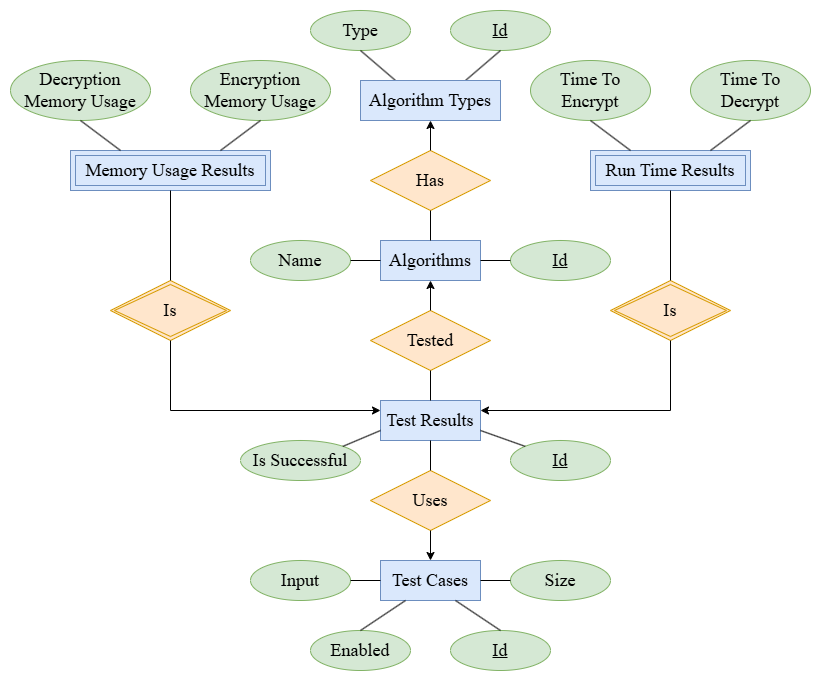
\includegraphics[width=0.8\textwidth]{Figures/EntityRelationship.png} % Kép beszúrása.
    \caption{Az adatbázis egyed-kapcsolat diagramja} % Az ábra neve.
    \label{fig:EntityRelationship} % Az ábra referenciája.
\end{figure}

\section{Eredmények megjelenítése} % Sorszámozott alcím létrehozása.

Az eredeti elképzelésemben táblázatokban akartam összegyűjteni a tesztek eredményeit. Egy táblázat lett volna a futási idő teszteredményeknek, egy másik pedig a memóriahasználat eredményeknek. Gyorsan be kellet látnom, hogy így nagyon nehezen áttekinthetőek az adatok. Ami részben abból eredt, hogy a különböző fajta algoritmusok együtt vannak megjelenítve. Ezért áttértem inkább a diagramokra, azon belül is a vonaldiagramra. Ez határozottan jobb megoldás volt, így sokkal áttekinthetőbbek lettek az eredmények.

A diagram X tengelyén a tesztelt bemenet mérete van bájtban. Az Y tengelyen pedig a teszt eredménye. Az algoritmusonként megjelenő több vonal elkerülése érdekében az egyes teszteredmények pontdiagramként vannak kirajzolva. Majd ezek átlagolva lesznek minden egyes X tengelyen lévő értékben. Ezzel biztosítva, hogy algoritmusonként csak egy egyenes jelenik meg.

A végleges verzió szerint minden algoritmus egyetlen diagramon fog megjelenni. Mindegyikhez hozzá van rendelve egy szín, amivel az a konkrét algoritmus ábrázolva van a diagramon. Az ábra túlzsúfolásának elkerülése érdekében meg lehet adni szűrési feltételeket a megjelenítendő teszteredményekre. Ilyen például az algoritmus típusa, a tesztelt tulajdonság vagy az algoritmus neve. Ezek segítségével csökkenteni lehet az ábrán megjelenítendő adatokat, ez által átláthatóbbá téve azt.

\chapter{Megvalósítás} % Sorszámozott fejezet létrehozása.

\section{Az alkalmazás alapjai} % Sorszámozott alcím létrehozása.

Mivel minden részt külön osztálykönyvtárba helyeztem, ezért az áttekinthetőség kedvért készítettem egy \textit{Directory.Packages.props} fájlt a NuGet csomagok központosított kezelésére. Így az összes csomag verziója egységes az egész projekten keresztül. A fájl pontos tartalma a \ref{fig:Implementation1} ábrán látható. Megfigyelhető, hogy a fájl elején lévő beállítást igazra állítottam. Ez azért történt így, mert ennek köszönhetően a fordító hibát fog dobni, ha valamelyik osztálykönyvtárban megpróbálok egy csomag verziót definiálni. Ez által garantálva, hogy nem lesz verzióeltérés a NuGet csomagok között.

% Kötelező helyű ábra beszúrása.
\begin{figure}[H]
    \centering % Az ábra középre igazítása.
    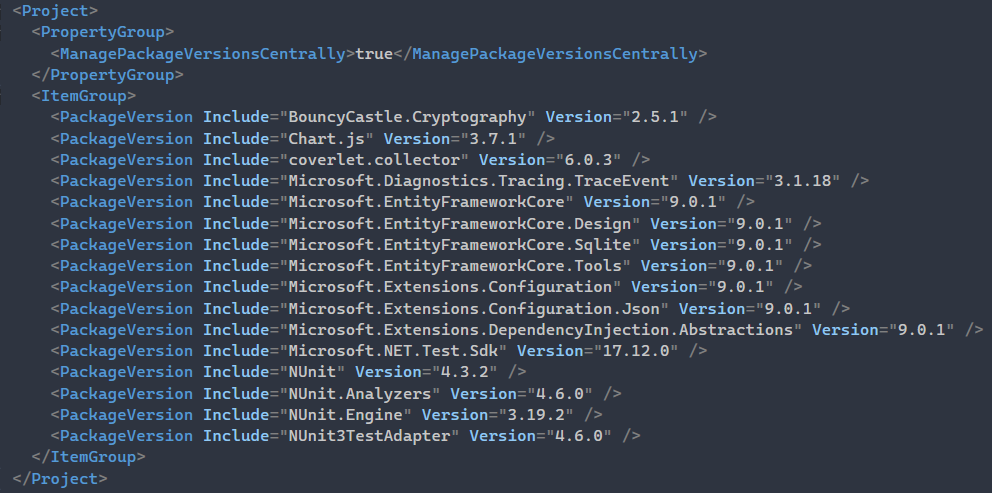
\includegraphics[width=0.8\textwidth]{Figures/Implementation1.png} % Kép beszúrása.
    \caption{A Directory.Packages.props fájl tartalma} % Az ábra neve.
    \label{fig:Implementation1} % Az ábra referenciája.
\end{figure}

Szükségesnek éreztem készíteni az alkalmazás számára egy központi \textit{appsettings.json} fájlt is. Ide kerül minden beállítás ami több mint egy osztálykönyvtárt érint. Továbbá aki jártasabb az ASP.NET Core webalkalmazásokban az tudja, hogy minden alkalmazásnak automatikusan generálódik egy \textit{appsettings.json} és egy \textit{appsettings.Development.json}. Figyelembe véve, hogy nekem már van egy központilag elérhető ilyen jellegú fájlom, ezért ezt a két automatikusan létrehozott fájl töröltem. Valamit a könnyebb és egységes kezelhetőség érdekében készítettem egy \textit{GlobalConfiguration} statikus osztályt, amely teljesen elrejti az \textit{appsettings.json} fájt. Ez az osztály fogja kiszolgálni a program minden részét, ami szeretne valamilyen információt a konfigurációs fájlból. Ez által biztosítva, hogy a futás közben történő konfigurációs fájl módosítása esetén mindenhol észlelődik a változtatás. Továbbá, hogy soha nem lesz két azonos példány beolvasva az \textit{appsettings.json} fájlból a memóriába. Értelem szerűen az ASP.NET Core alkalmazásnak is ő adja át a konfigurációs fájlt.

\section{Algoritmusok} % Sorszámozott alcím létrehozása.

\section{NUnit tesztek} % Sorszámozott alcím létrehozása.

\section{Tesztesetek automatizálása} % Sorszámozott alcím létrehozása.

\section{Adattárolás} % Sorszámozott alcím létrehozása.

\section{A webalkalmazás} % Sorszámozott alcím létrehozása.

\section{Tesztek integrálása} % Sorszámozott alcím létrehozása.

\section{Eredmények megjelenítése} % Sorszámozott alcím létrehozása.

\chapter{Saját algoritmus} % Sorszámozott fejezet létrehozása.

\section{Elképzelés} % Sorszámozott alcím létrehozása.

Az alap ötletem az volt, hogy egy algoritmus kulcsának növelésével csökkenthetjük az elvégezendő műveletek számát. Ez által csökkenne a futáshoz szükséges idő. Ehhez plusz információval kell ellátnunk a kulcsot, szóval az eddigi kulcsok felépítése nem fog működni. Viszont továbbra is szeretném, hogy a kulcsot ki lehessen exportálni szöveges fájlként.

Mivel ez lesz az első ilyen próbálkozásom, ezért egy szimmetrikus kulcsú titkosító algoritmust szeretnék készíteni. Személyes meglátásom alapján ezt a legkönnyebb megvalósítani. Jelentősebben egyszerűbb, mint egy aszimmetrikus kulcsú algoritmust. A hasító algoritmusokról nem is beszélve, talán azokat a legnehezebb elkészíteni.

\section{A fejlődés folyamata} % Sorszámozott alcím létrehozása.

Az első ötletem az volt, hogy egyszerűen vektorok összegeként titkosítom a szöveget. Az ihletet a vektorok összeadása adta, hiszen ott sem látszik, hogy melyik két komponens vektor összege az eredmény vektor. De ugye ehhez le kell tudnunk méri a vektorok pontos adatait. Itt jöttem rá, hogy a kulcs lehetne egy koordináta-rendszer és minden betűt egy pontként ábrázolnánk benne. A programkódban ez egy kétdimenziós karakter tömb lenne, ahol az X és Y koordinátáknak a tömbelem két indexe felel meg. Az \ref{fig:MyAlgorithm1} ábrán látható egy példa, hogy hogyan nézhet ki egy kulcs. Itt a karakterek éppen a magyar ábécé nagy betűi, de értelem szerűen bármilyen karakterek lehetnek, bele értve a vezérlő karaktereket is.

% Kötelező helyű ábra beszúrása.
\begin{figure}[H]
    \centering % Az ábra középre igazítása.
    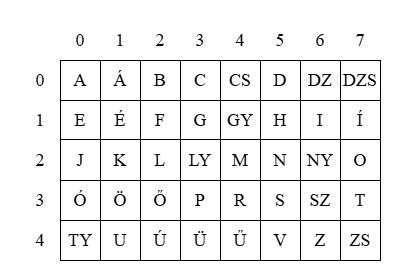
\includegraphics[width=0.6\textwidth]{Figures/MyAlgorithm1.png} % Kép beszúrása.
    \caption{A magyar ábécé nagy betűit tartalmazó kulcs} % Az ábra neve.
    \label{fig:MyAlgorithm1} % Az ábra referenciája.
\end{figure}

Sajnos már az első alkalommal problémába ütköztem, amikor titkosítani akartam egy szöveget ezzel a kulccsal. Az irányított vektorok nem a voltak a leghatékonyabb módjai az ehhez hasonló tömbökön történő mozgásnak. Ekkor jutott eszembe, hogy fizikában is mindig szétbontjuk a vektorokat olyan komponensekre, amelyek iránya és irányítása megegyezik a koordináta rendszer tengelyeivel. Én is ezt tettem, egy-egy külön vektort használtam a vízszintes és a  függőleges mozgás jelölésére. Tehát az előbb említett módszerrel, az \ref{fig:MyAlgorithm1} ábrán látható kulccsal, az N betű titkosítása az 5 egység hosszú vízszintes és 2 egység hosszú függőleges vektor lenne. A sorrend természetesen mindegy, mert a vektorok összeadása kommutatív.

Mivel egy szónak csak úgy van értelme, hogy a betűk a megfelelő sorrendben következnek egymás után. Ezért arra gondoltam, hogy a vektorok mindig az előző betű pozíciójából indulnak. Ez által nehezítve a visszafejtést. Az átláthatóság kedvért mindig a vízszintes vektor van elsőként írva. Továbbá az egyszerűbben áttekinthető forma érdekében, a két vektor $(\text{vízszintes} \mid \text{függőleges})$ alakban van elrendezve.

% Kötelező helyű ábra beszúrása.
\begin{figure}[H]
    \centering % Az ábra középre igazítása.
    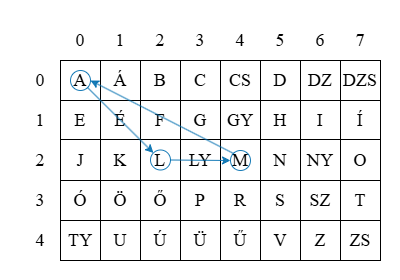
\includegraphics[width=0.6\textwidth]{Figures/MyAlgorithm2.png} % Kép beszúrása.
    \caption{Az ALMA szó titkosítása az adott kulcson} % Az ábra neve.
    \label{fig:MyAlgorithm2} % Az ábra referenciája.
\end{figure}

Az \ref{fig:MyAlgorithm2} ábrán látható az ALMA szó titkosításának lépései. Az első lépés az A betű titkosítása, ami egyszerűen $(0 \mid 0)$ lesz. Ez után el kell jutnunk az L betűbe, ehhez kell két darab 2 egység hosszú vektor, vagyis $(2 \mid 2)$. A következő célpont az M betű. Mivel már a megfelelő sorban vagyunk, ezért csak vízszintes vektor kell. Tehát az esetünkben $(2 \mid 0)$ lesz a megoldás. Végül vissza kell jutnunk az A betűbe. Ehhez a szükséges vektorok $(-4 \mid -2)$ lesznek. Mind ezt összegezve, az eredményünk a $(0 \mid 0), (2 \mid 2), (2 \mid 0), (-4 \mid -2)$ vektorok sorozata lesz.

A következő módosítás amit véghez vittem, a kulcs végtelenítése volt. Ezt úgy kell érteni, hogy az algoritmus szabadon lesétálhat a kulcsról. Amikor ez bekövetkezik, akkor a kulcs átellenes oldalára kerül. Ez azt jelenti, hogy az \ref{fig:MyAlgorithm2} ábrán az algoritmus az O betűből el tud jutni a J betűbe egy $(1 \mid 0)$ mozgással. Ennek tudatosan nincs jelölése a végeredményben, ezzel is bonyolítva a titkosított szöveg illetéktelen visszafejtését.

Támadt egy olyan ötletem, hogy egy karakter akár többször is szerepelhetne a kulcsban. Az algoritmus pedig véletlenszerűen választana egyet, majd annak a pozícióját használná a vektorok elkészítéséhez. Ezzel a megoldással egy betűt több különböző módon lehet titkosítani, ezzel növelve a biztonságot.

Ekkor szembesültem vele, hogy az algoritmus futási ideje borzasztó. Az oka pedig, hogy minden lépés előtt, meg kell vizsgálnia az egész kulcsot, hogy hol található a kövekező betű, ahova el kell jutnia. Ezen úgy sikerült túllépni, hogy a kulcs beállítása után az algoritmus készít magának egy szótárat róla. A szótárban szereplő kulcsok az algoritmus kulcsában megtalálható karakterek, az értékek pedig az előfordulásuk pozícióinak listája. Ezzel jelentősen sikerült lecsökkenteni az algoritmus futási idejét.

A titkosított szöveg még mindig elég sok információt tartalmazott. Például, hogy hány karakterből állt az eredeti szöveg. Drasztikus lépésnek tűnhet, de egyszerűen kivettem minden jellegű tagolást a titkosított szövegből. Viszont így már nem lehetett vissza fejteni. Ezért arra gondoltam, hogy standardizálom a vektorok méretét a kulcs mérete alapján. Ezt azt jelenti, hogy egy kétszámjegyű magasságú kulcson a függőleges vektorok mindig két számjeggyel lesznek ábrázolva. Ugyan ez érvényes a kulcs szélességére és a vízszintes vektorokra is. Ezzel a módosítással az \ref{fig:MyAlgorithm2} ábrán látható ALMA szó titkosítása az adott kulccsal $002220-4-2$ lesz.

Jól látható, hogy a negatív számok még mindig sok információt adhatnak az eredeti szövegről. A megoldás viszont nagyon egyszerű a problémára. Mind össze le kell korlátozni, hogy az algoritmus nem léphet negatív irányba. Szerencsére ez nem probléma, mivel a végtelenített kulcsnak köszönhetően így is el tud jutni minden karakterbe. Így most már az ALMA szó titkosítása $00222043$ lesz. A módosított algoritmus lépései az \ref{fig:MyAlgorithm3} ábrán láthatóak. Jól megfigyelhető, hogy az algoritmus csak jobbra és lefelé léphet. Ez a már előbb említett negatív számok elkerülése miatt szükséges.

% Kötelező helyű ábra beszúrása.
\begin{figure}[H]
    \centering % Az ábra középre igazítása.
    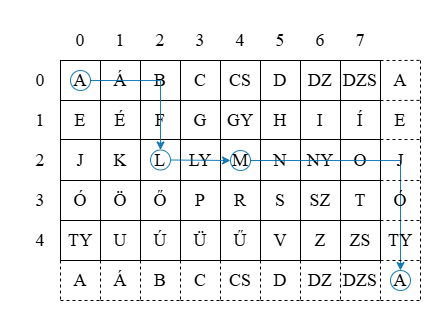
\includegraphics[width=0.6\textwidth]{Figures/MyAlgorithm3.png} % Kép beszúrása.
    \caption{Az ALMA szó titkosítása a módosított algoritmussal} % Az ábra neve.
    \label{fig:MyAlgorithm3} % Az ábra referenciája.
\end{figure}

Ahogy tesztelgettem az algoritmust, arra lettem figyelmes, hogy a futási idő jelentős részét a véletlen karakter választása teszi ki. Azt egy saját lista kollekció megvalósításával tudtam orvosolni. Ez a lista továbbra is a karakterek előfordulását tárolja, viszont eltárolja az utoljára visszaadott elem indexét is. Valamint van egy plusz függvénye, ami az eltárolt index szerint visszaadja a következő elemet, majd megnöveli az indexet egyel. Ha az index eléri a lista végét, akkor a kollekció megkeveri az elemeit, majd az indexet az első elemre állítja. Ez által gyorsítva az algoritmus futását. Valamint garantálva, hogy a többször szereplő karakterek ki is vannak használva, nem csak felesleges helyet foglalnak a kulcsban.

\section{Jelenlegi állapot} % Sorszámozott alcím létrehozása.

Szerintem az algoritmus jelenleg egy nagyon stabil állapotában van. Véleményem szerint nem sok kellene neki, hogy versenyezni tudjon a napjainkban használt algoritmusokkal. Egy mindennapi használatra alkalmas kulcsot láthatunk az \ref{fig:MyAlgorithm4} ábrán. Igaz, ez a kulcs nem alkalmas magyar szövegek titkosítására, mivel nem tartalmaz magyar ékezetes betűket. Ennek ellenére egy általános angol nyelű dokumentumot gond nélkül tud titkosítani.

% Kötelező helyű ábra beszúrása.
\begin{figure}[H]
    \centering % Az ábra középre igazítása.
    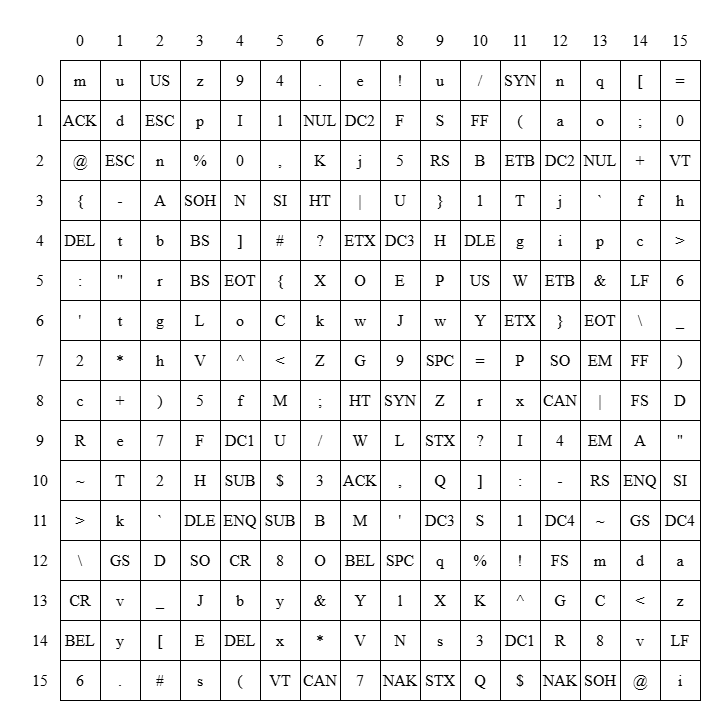
\includegraphics[width=0.8\textwidth]{Figures/MyAlgorithm4.png} % Kép beszúrása.
    \caption{Egy mindennapi használatra alkalmas kulcs} % Az ábra neve.
    \label{fig:MyAlgorithm4} % Az ábra referenciája.
\end{figure}

A mostani megvalósítás a MathCrypt nevet viseli. A pontos szerkezete az \ref{fig:MyAlgorithm5} ábrán látható. A könnyebb használat érdekében készítettem egy kulcs generátort is. Az \ref{fig:MyAlgorithm4} ábrán látható kulcsot is ezzel hoztam létre. Valamint mind az algoritmus, mind a generátor rendelkezik interfésszel a jövőbeli fejlesztések megkönnyítése érdekében. A \textit{SPoint} egy egyszerű koordinátát ábrázoló struktúra. A \textit{ShuffleList} pedig a már korábban említett beépített keveréssel rendelkező saját lista kollekcióm.

% Kötelező helyű ábra beszúrása.
\begin{figure}[H]
    \centering % Az ábra középre igazítása.
    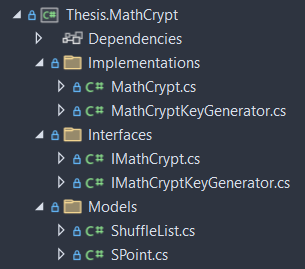
\includegraphics[width=0.5\textwidth]{Figures/MyAlgorithm5.png} % Kép beszúrása.
    \caption{A megvalósított algoritmus szerkezete} % Az ábra neve.
    \label{fig:MyAlgorithm5} % Az ábra referenciája.
\end{figure}

\section{Jövőbeli tervek} % Sorszámozott alcím létrehozása.

Az algoritmusom rengeteg változtatáson ment már keresztül. Ennek ellenére még közel sincs készen. Itt most nem arra gondolok, hogy teljesítményben lemaradottabb a versenytársaival szemben. Hanem a lehetséges fejlesztési irányokra és funkciókra.

Az egyik ilyen ötletem lehetővé tenné, hogy visszafejtés nélkül megváltoztatjuk a szöveget kódoló kulcsot. Nem olyan értelemben, hogy egy teljesen más kulccsal lehetne elolvasni. Ez integritás szempontjából nem lenne a legjobb döntés. Itt arra kell, gondolni, hogy egy módosító számmal el lehet tolni a már lekódolt szöveg számjegyeit. Valamint ezzel a számmal el kell tolni a kulcs sorait és oszlopait is. Kicsit úgy mint ha a kulcs egy Rubik kocka lenne. Gyalogosan papíron már próbáltam és működik. Viszont a programkód megvalósítása lehet nem lesz a legegyszerűbb. Továbbá meg kell vizsgálni, hogy pontosan milyen hatásokat válthat ki a funkció megvalósítása. Esetlegesen törhetőbbé teszi-e az algoritmust vagy idéz-e valamit más nemkívánatos hatást.

Van még ehhez hasonló pár ötletem az algoritmus javítására. De sajnos a szűkös időkorlát nagyban limitálta az algoritmus fejlődését. Minden esetre nagyon élveztem a fejlesztést. Nem bántam meg, hogy belevágtam a kihívásba.

\chapter{Teszteredmények} % Sorszámozott fejezet létrehozása.

\section{Szimmetrikus algoritmusok} % Sorszámozott alcím létrehozása.

\section{Aszimmetrikus algoritmusok} % Sorszámozott alcím létrehozása.

\section{Hasító algoritmusok} % Sorszámozott alcím létrehozása.

\section{A saját algoritmusom} % Sorszámozott alcím létrehozása.

\chapter{Összefoglalás} % Sorszámozott fejezet létrehozása.

\chapter*{Irodalomjegyzék} % Sorszámozott fejezet létrehozása.
\addcontentsline{toc}{chapter}{Irodalomjegyzék} % A fejezet hozzáadása a tartalomjegyzékhez.

\printbibliography[heading=none] % A citerált irodalmak kilistázása.

\chapter*{Nyilatkozat} % Sorszámozott fejezet létrehozása.
\addcontentsline{toc}{chapter}{Nyilatkozat} % A fejezet hozzáadása a tartalomjegyzékhez.

Alulírott Molnár Gábor Ádám, programtervező informatikus BSc szakos hallgató, kijelentem, hogy a dolgozatomat a Szegedi Tudományegyetem, Informatikai Intézet Szoftverfejlesztés Tanszékén készítettem, programtervező informatikus BSc diploma megszerzése érdekében.

Kijelentem, hogy a dolgozatot más szakon korábban nem védtem meg, saját munkám eredménye, és csak a hivatkozott forrásokat (szakirodalom, eszközök stb.) használtam fel.

Tudomásul veszem, hogy szakdolgozatomat a Szegedi Tudományegyetem Diplomamunka Repozitóriumában tárolja.

\vspace{1cm}

{\large Kelt.: 2025. május 13.}

\vspace{0.5cm}
\hfill
\parbox{5cm}{\centering\hrule\vspace{0.3cm} Aláírás}

\end{document} % A dokumentum vége.
